% !TeX root = ./kernel/EasySolution.tex
\section*{Solution de l'exercice 1 \MarksTwo}

\begin{enumerate}
      \item Décrivez brièvement le fonctionnement d'un réseaux intélligent.
            \begin{itemize}
                  \item Les réseaux intelligents fonctionnent principalement avec des capteurs et objets connectés placés dans / sur des infrastructures physiques. Ces capteurs vont alors émettre des données qui vont remonter à l’aide d’un réseau sans fil sur des plateformes de réseaux intelligents. Elles pourront être ainsi analysées et enrichies pour en tirer le meilleur profit. Ces plateformes de data management et de data visualisation sont les nouvelles solutions intelligentes permettant aux territoires, entreprises ou même usagers d’analyser les données et d’en tirer des conclusions pour pouvoir adapter pratiques et comportements.
            \end{itemize}
      \item Donner la représentation de l’architecture d’un projet réseau intelligent.
            \begin{itemize}
                  \item Voir la figure \ref{fig:arch}
            \end{itemize}
            \begin{figure}[!ht]
                  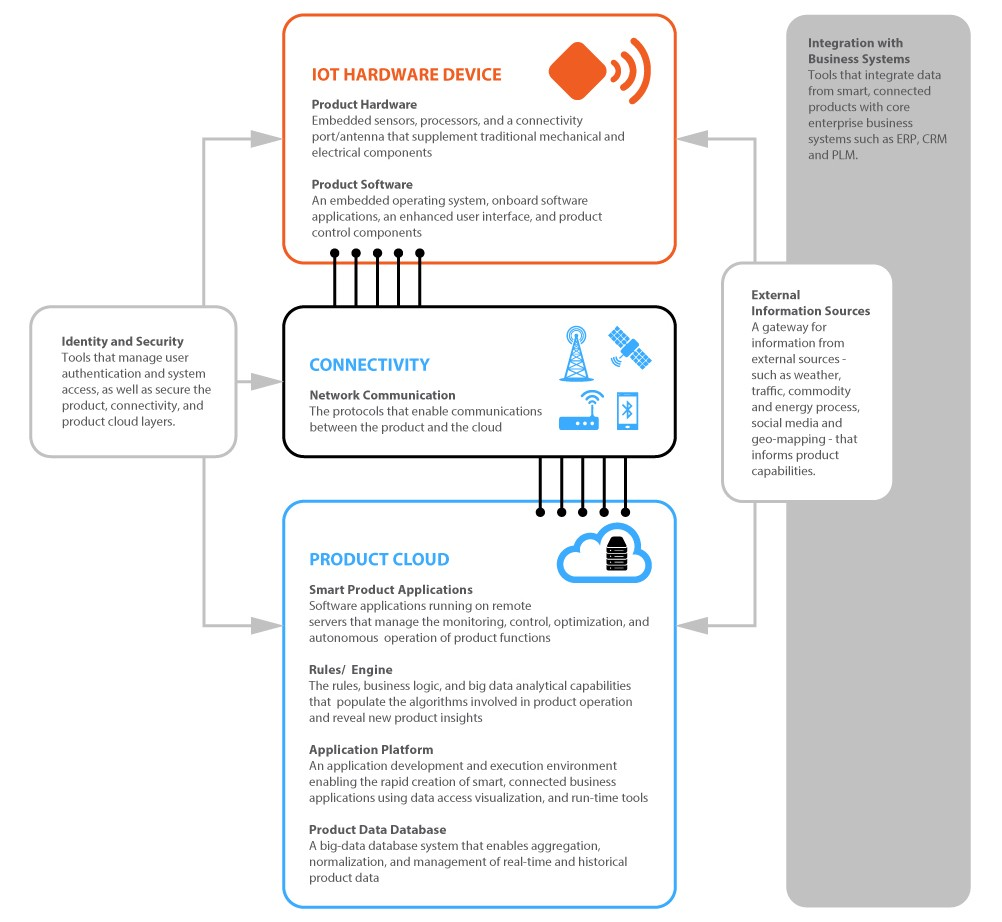
\includegraphics[trim={1cm, 0cm, 0cm, 0cm}, width=18cm, clip]{../../figs/iot_arch.jpeg}
                  \caption{Représentation de l'architecture d'un projet de réseau intélligent.}
                  \label{fig:arch}
            \end{figure}
      \item Citez en donnant les fonctions de chaque couches de l'architecture des réseaux intélligents.
            \begin{itemize}
                  \item  Composant hardware : le dispositif physique qui interagit avec l’environnement.
                  \item Connectivité : le lien entre votre appareil et le cloud
                  \item produits du cloud : serveurs qui prennent des données, les traitent, les
                        stockent dans des bases de données, donnent des commandes, effectuent
                        des analyses, servent les données de manière utile à tous les différents
                        acteurs.
            \end{itemize}
      \item Citez 05 (cinq) protocoles des réseaux intélligents.
            \begin{itemize}
                  \item Bluetooth
                  \item LoRaWAN
                  \item RFID/NFC
                  \item WiFi
                  \item 6LoWPAN
            \end{itemize}
      \item Quelle est la couche de l'architecture des réseaux intélligents qui interagit directement avec les processus industriels ?
            \begin{itemize}
                  \item Couche Hardware ou matériel.
                  \item Cette interaction se fait à travers de capteurs et actionneurs.
            \end{itemize}
      \item Donnez la différence entre un réseaux dit "non intélligent" et un réseaux intélligent.
            \begin{itemize}
                  \item{Les réseaux intelligents sont des réseaux matériels de distributions de fluides (électricité, eau, gaz, pétrole...), et/ou d'information (télécommunications) qui ont été « augmentés » (rendus intelligents) par des systèmes informatiques, capteurs, interfaces informatiques et électromécaniques leur donnant des capacités d'échange bidirectionnel et parfois une certaine capacité d'autonomie en matières de calcul et gestion de flux et traitement d'information.}
            \end{itemize}
\end{enumerate}